\section{Back end}
\subsection{Descrizione generale}
\subsubsection{Comunicazione tra client e server}
Per la creazione del back end di MaaS si è deciso di utilizzare Node.js e, in particolare, il framework ExpressJS, che permette la creazione semplificata di server REST. Il lato back end sarà quindi costituito da un insieme di API protette da strati diversi di sicurezza. \\
Ciascuna API del webserver fornirà una risposta in formato JSON per permettere la fruizione delle informazioni. Fornirà nello stesso formato anche gli eventuali messaggi di errore generati nel corpo dei metodi del server. Tali messaggi di errore saranno così composti: 
\begin{verbatim}
{
    "code":     [Codice definito nel protocollo HTTP, che identifica univocamente
                 la tipologia del problema]
    "message":  [Messaggio che definisce in dettaglio la tipologia dell'errore]
    ["data":   [Opzionale, trasporta i dati in cui si è verificato l'errore]]
}
\end{verbatim}
I codici di errore saranno del tipo 4xx (client error, la richiesta è sintatticamente scorretta o non può essere soddisfatta) o 5xx (server error, il server ha fallito nel soddisfare una richiesta apparentemente valida).
\subsubsection{Sicurezza}
Gli accessi alle API avranno 2 livelli di sicurezza. \\
Il primo livello è rappresentato dall'autenticazione: un utente non autenticato riceverà un errore se richiede una API protetta. Verrà implementato con l'utilizzo di PassportJS, un middleware per ExpressJS che permette l'autenticazione di utenti nel sistema. In particolare verrà utilizzata la strategia passport-local per l'accesso al server, cioè le credenziali dell'utente risiederanno nel database locale. \\
Il secondo livello è definito in base al ruolo di appartenenza di un utente. Si occuperà di controllare i permessi assegnati ad un utente autenticato e di verificare la possibilità che possa o meno interagire con la risorsa richiesta. \\
I ruoli utente ammessi nell'applicazione sono: 
\begin{itemize}
\item \textbf{GUEST};
\item \textbf{MEMBER};
\item \textbf{ADMIN};
\item \textbf{OWNER};
\item \textbf{SUPERADMIN}.
\end{itemize}
Per il ruolo di SUPERADMIN è abilititato un set di API per la gestione dell'intera applicazione. Tali API non sono accessibili agli utenti con altri ruoli.
\subsection{Package e classi}
\begin{figure}[h]
\centering
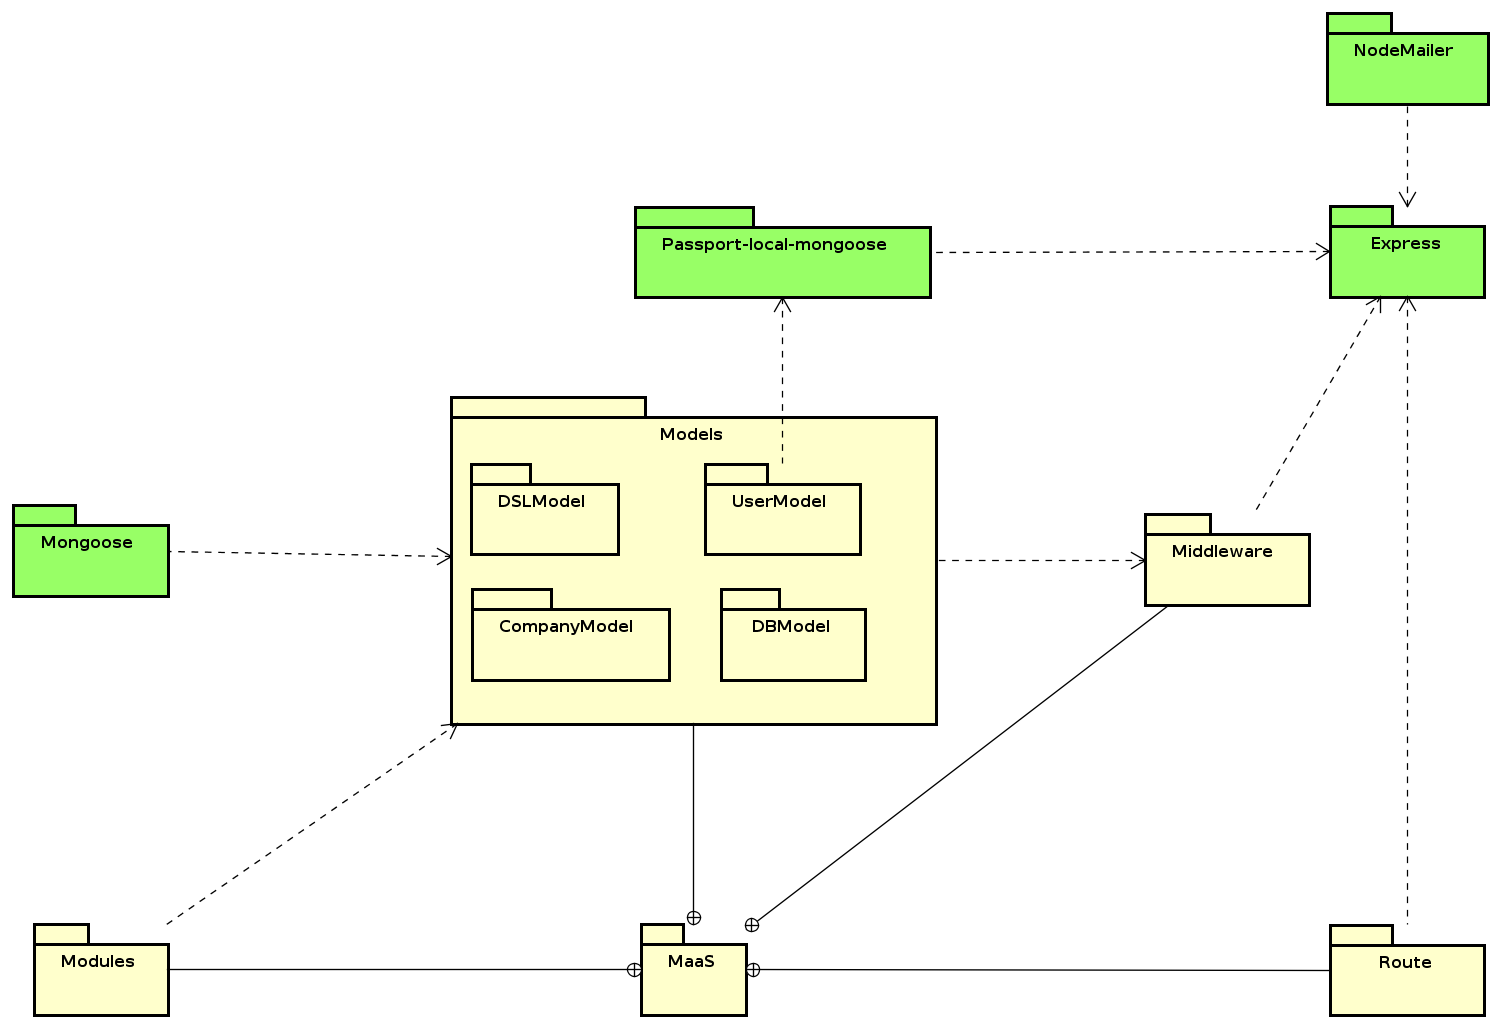
\includegraphics[width=0.8\textwidth]{res/sections/package.png}
\caption{Diagramma dei package per il backend}
\end{figure}
\subsubsection{Middleware}
\paragraph{Descrizione}
In questo package è contenuto il modulo che verifica se il ruolo dell'utente gli permette di eseguire l'operazione richiesta.
\paragraph{Moduli contenute}
\subparagraph{LevelChecker}
\begin{description}
\item[Descrizione] \hfill \\
Questo è il modulo che controlla se il ruolo dell'utente gli permette di eseguire l'operazione richiesta.
\item[Utilizzo] \hfill \\
Viene utilizzato per implementare il secondo livello di sicurezza dell'applicazione. Ad ogni richiesta il cui esito varia in base al ruolo

\subsubsection{Models}
%todo immagine interazioni tra i modelli
\paragraph{Descrizione}
In questo package sono definiti i modelli di dato che rappresentano il core business dell'applicazione:
\begin{itemize}
\item User;
\item Company;
\item DSL;
\item Database;
\end{itemize}
\paragraph{Package contenuti}
\begin{itemize}
\item UserModel;
\item CompanyModel;
\item DSLModel;
\item DatabaseModel;
\end{itemize}

\subsubsection{Modules}
%todo diagramma delle classi
\paragraph{Descrizione}
In questo package sono contenute tutte le utility utilizzate dall'applicazione.
\paragraph{Classi contenute}
\subparagraph{PermissionChecker}
\begin{description}
\item[Descrizione] \hfill \\
Questa classe si occupa di controllare che un utente abbia il permesso di eseguire un'operazione su una specifica DSL.
\item[Utilizzo] \hfill \\
Viene utilizzata per capire se consentire o meno l'accesso in esecuzione o scrittura ad una specifica DSL.
\end{description}
\subparagraph{DSLChecker}
\begin{description}
\item[Descrizione] \hfill \\
%todo
\item[Utilizzo] \hfill \\
%todo
\end{description}

\subsubsection{Route}
\paragraph{Descrizione}
In questo package sono presenti tutti i moduli contenenti le varie Routes. In ExpressJS, il routing ha il compito di determinare come l'applicazione risponde ad una richiesta del client verso un particolare endpoint. L'endpoint è semplicemente una coppia formata da un URI e da un metodo di richiesta (GET, POST, PUT o DELETE). Ogni route può avere una o più funzioni associate che bengono eseguite quando la route è invocata.
\paragraph{Classi contenute}
%todo

\subsubsection{UserModel}
%todo immagine UserModel
\paragraph{Descrizione}
In questo package sono contenute le classi che modellano gli utenti.
\paragraph{Classi contenute}
\subparagraph{User}
\begin{description}
\item[Descrizione] \hfill \\
Questa classe modella il concetto di utente, 
\item[Utilizzo] \hfill \\
\end{description}
\subsubsection{CompanyModel}
\paragraph{Descrizione}
\paragraph{Classi contenute}

\subsubsection{DSLModel}
\paragraph{Descrizione}
\paragraph{Classi contenute}

\subsubsection{DBModel}
\paragraph{Descrizione}
\paragraph{Classi contenute}